\documentclass{article}%
\usepackage[T1]{fontenc}%
\usepackage[utf8]{inputenc}%
\usepackage{lmodern}%
\usepackage{textcomp}%
\usepackage{lastpage}%
\usepackage[head=40pt,margin=0.5in,bottom=0.6in]{geometry}%
\usepackage{graphicx}%
%
\title{\textbf{Detuvieron a ocho funcionarios de la CPNB por homicidio en El Valle}}%
\author{El Nacional Web | Con información de Sandra Guerrero}%
\date{06/12/2018}%
%
\begin{document}%
\normalsize%
\maketitle%
\textbf{URL: }%
http://www.el{-}nacional.com/noticias/sucesos/detuvieron{-}ocho{-}funcionarios{-}cpnb{-}por{-}homicidio{-}valle\_262324\newline%
%
\textbf{Periodico: }%
EN, %
ID: %
262324, %
Seccion: %
Sucesos\newline%
%
\textbf{Palabras Claves: }%
Tiroteo, Sucesos, Caracas\newline%
%
\textbf{Derecho: }%
1.1, %
Otros Derechos: %
1.10, %
Sub Derechos: %
1.1.1.9, 1.10.1\newline%
%
\textbf{EP: }%
NO\newline%
\newline%
%
\textbf{\textit{En el suceso falleció un hombre de 17 años de edad además de dos personas heridas de 13 y 17 años ~}}%
\newline%
\newline%
%
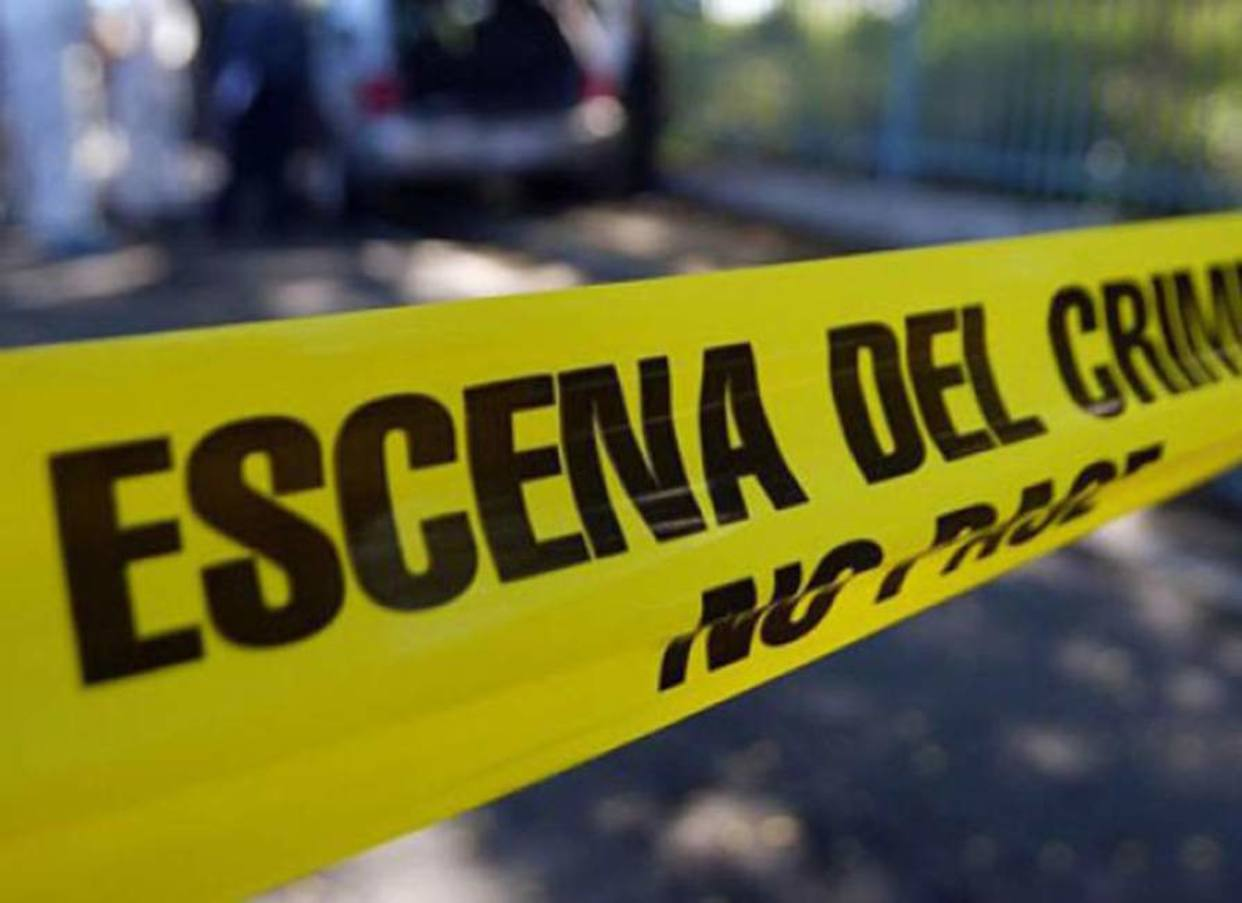
\includegraphics[width=300px]{16.jpg}%
\newline%
%
Ocho funcionarios del Cuerpo~la Policía Nacional Bolivariana (CPNB) y una persona fueron detenidas por el homicidio de un hombre y por ocasionar lesiones graves a otras tres personas.%
\newline%
%
La víctima tenía 17 años de edad y entre las personas heridas hay dos jóvenes de 13~ y 17 años. Otro de los heridos, que tenía 12 años, falleció este jueves.~El hecho ocurrió este miércoles en la avenida intercomunal de El Valle en la calle 18 a las 10:00 pm.%
\newline%
%
Seis de de los funcionarios pertenecen a la estación policial de El Valle y los otros dos están adscritos a la dirección de casos especiales de la Fuerza de Acciones Especiales de la Policía Nacional Bolivariana.%
\newline%
%
\end{document}